\documentclass{article}

\usepackage[utf8]{inputenc}
\usepackage[T1]{fontenc}
\usepackage[francais]{babel}
\usepackage{url}
\usepackage{color}
\usepackage{verbatim}
\usepackage{amsmath,amssymb,amsfonts}
\usepackage{graphicx}
\usepackage[french]{algorithm2e}
\usepackage{geometry}
\usepackage{enumitem}
\usepackage{listings}
\usepackage{listingsutf8}
\usepackage{caption}
\captionsetup[figure]{slc=on}
\frenchbsetup{StandardLists=true}
\lstset{language=Java}
\lstset{
	breaklines=true, 
	showspaces=false, 
	keepspaces=true, 
	numbers=left, 
	frame=single, 
	keywordstyle=\color{blue},
	basicstyle=\ttfamily\small,
	commentstyle=\color{green}
}
\geometry{hmargin=2.5cm, vmargin=2.5cm}

\title{Conception des Systèmes d'Exploitation\\Rapport sur les mesures expérimentales du tri}
\author{Line \bsc{POUVARET}, Mickaël \bsc{TURNEL}}
\date{2015-2016}

\begin{document}
\maketitle

\section{Réponses aux Questions du TP}

\subsection*{Question 1}

Il est judicieux de placer les appels à gettimeofday juste avant et après l'exécution de l'algorithme de tri.\\

En particulier, il est nécessaire d'inclure la création de threads et la synchronisation finale dans la mesure du temps car il nous faut savoir combien de temps met le programme à créer ses threads et à les synchroniser.

\subsection*{Question 2}

Oui l'ordonnanceur a une influence sur le programme car gettimeofday nous permet de mesurer un temps absolu alors que l'ordonnanceur a peut être donné la main à un autre programme pendant la mesure du temps.

\subsection*{Question 3}

Oui le nombre de threads influe sur le temps reporté par getrusage puisque cette fonction calcule le cumul du temps passé par chaque thread
du programme.\\

Donc, plus on créera de threads, et plus le temps reporté par getrusage sera grand.\\

Si on crée plus de threads que de nombre de processeurs (ou coeurs) alors les threads ne seront pas tous exécuté en parallèle mais cela 
n'influence pas plus ou moins sur le temps reporté par getrusage.\\

En revanche, cela influe énormément sur le temps écoulé depuis le début
du lancement du programme.


\subsection*{Question 4}

Puisque l'algorithme s'éxécute de façon parallèle grâce aux threads, le temps correspondant au cumul de l'ensemble des threads du processus 
obtenu avec getrusage sera forcément supérieur au temps obtenu avec gettimeofday (sauf si l'on exécute un seul thread uniquement, dans ce cas,
le temps obtenu avec getrusage est légèrement inférieur à celui obtenu avec gettimeofday).

\subsection*{Question 5}

Influences sur l'accélération et l'efficacité d'un programme parallèle :

\begin{itemize}
	\item algorithmes utilisés $\rightarrow$ influe sur l'accélération et l'efficacité car cela va dépendre de la complexité de l'algorithme, des accès mémoires,
		opérations arithmétiques, etc...L'accélération va diminuer plus l'algorithme sera complexe et utilisera des instructions coûteuses en temps.
		Donc l'efficacité va diminuer aussi.
	\item nombre de threads utilisés $\rightarrow$ influe sur l'accélération et l'efficacité car un programme parallèle qui utilise un nombre de threads inférieur à
		celui d'un autre programme parallèle sera plus long. Par contre utiliser un nombre de thread supérieur au nombre de coeurs du processeur
		donnera lieu à un temps d'exécution plus long.
	\item bibliothèque de threads utilisée $\rightarrow$ influe probablement puisqu les bibliothèques de threads ont des fonctionnement différents
	\item le système d'exploitation $\rightarrow$ ne doit pas influer sur ces deux critères
	\item le nombre de processeurs de la machine $\rightarrow$ influe sur l'accélération et l'efficacité car si l'algorithme utilise par exemple un trop grand nombre de threads, le processeur va passer beaucoup de temps à passer d'un thread à un autre
	\item la vitesse des processeurs $\rightarrow$ influe, cela va de soit plus les processeurs seront rapides plus vite ils vont exécuter un algorithme
\end{itemize}

\section{Présentation du plan d'expérience}

Nous avons effectué nos tests sur la machine MandelBrot qui possède 4 processeurs.\\

Nous avons utilisé un script bash pour automatiser nos expériences et permettre de changer les paramètres (comme la taille du vecteur, le nombre de threads, le nombre de tests à effectuer...)\\

Nous avons effectué ce script bash avec un nombre de tests égal à 20 et récupéré les moyennes générées pour réaliser nos courbes.\\

\subsection*{Contenu de tri.sh}
\lstset{language=bash}
\begin{lstlisting}
#!/bin/bash

# On supprime les fichiers si il existe deja
rm -f resultat_sequentiel.txt resultat_thread.txt log_sequentiel.txt log_thread.txt

# Si on a pas le bon nombre d'arguments on indique comment utiliser la commande
if [ $# != 5 ]; then
        echo 'Usage : ./tri.sh <Nombre de test> <Taille du vecteur> <Min> <Max> <Nombre de threads>'
        exit
fi

# On cree notre vecteur
./creer_vecteur --size $2 --min $3 --max $4 > vecteur.txt

# On recupere le(s) resultat(s) du tri sequentiel dans le fichier log_sequentiel.txt
touch log_sequentiel.txt
for i in `seq 1 $1`;
do
        ./tri_sequentiel --quiet --time --rusage < vecteur.txt >> log_sequentiel.txt
done

# on recupere le(s) resultat(s) du tri avec threads dans le fichier log_thread.txt
touch log_threads.txt
for i in `seq 1 $1`;
do
        ./tri_threads --quiet --time --rusage --parallelism $5 < vecteur.txt >> log_thread.txt
done

# Puis on calcule la moyenne et on stocke le resultat dans le fichier resultat_sequentiel.txt
touch resultat_sequentiel.txt
i=1
while read aLine;
do
        tab[$i]=$aLine
        i=$(($i+1))
done < log_sequentiel.txt

count=$(($i-1))

counttime=1
countcpu=1
for i in `seq 1 $count`;
do
        if (( $i%2 != 0 )); then
                tabtime[$counttime]=${tab[$i]}
                counttime=$(($counttime+1))
        fi
        if (( $i%2 == 0 )); then
                tabcpu[$countcpu]=${tab[$i]}
                countcpu=$(($countcpu+1))
        fi
done

counttime=$(($counttime-1))
countcpu=$(($countcpu-1))

echo 'Temps global' >> resultat_sequentiel.txt

moyenne=0
for i in `seq 1 $counttime`;
do
        echo "Test $i : ${tabtime[$i]} micro secondes" >> resultat_sequentiel.txt
        moyenne=$(($moyenne+${tabtime[$i]}))
done
moyenne=$(($moyenne/$counttime))

echo "Moyenne (sur $counttime tests) : $moyenne" >> resultat_sequentiel.txt

echo 'Temps CPU' >> resultat_sequentiel.txt

moyenne=0
for i in `seq 1 $countcpu`;
do
        arr=(${tabcpu[$i]})
        echo "Test $i : ${arr[0]}" >> resultat_sequentiel.txt
        moyenne=$(($moyenne+${arr[0]}))
done
moyenne=$(($moyenne/$countcpu))

echo "Moyenne (sur $countcpu tests) : $moyenne" >> resultat_sequentiel.txt

# Puis on calcule la moyenne et on stocke le resultat dans le fichier resultat_thread.txt
touch resultat_thread.txt
i=1
while read aLine;
do
        tab[$i]=$aLine
        i=$(($i+1))
done < log_thread.txt

count=$(($i-1))

counttime=1
countcpu=1
for i in `seq 1 $count`;
do
        if (( $i%2 != 0 )); then
                tabtime[$counttime]=${tab[$i]}
                counttime=$(($counttime+1))
        fi
        if (( $i%2 == 0 )); then
                tabcpu[$countcpu]=${tab[$i]}
                countcpu=$(($countcpu+1))
        fi
done

counttime=$(($counttime-1))
countcpu=$(($countcpu-1))

echo "Avec $5 threads" >> resultat_thread.txt
echo 'Temps global' >> resultat_thread.txt

moyenne=0
for i in `seq 1 $counttime`;
do
        echo "Test $i : ${tabtime[$i]}" >> resultat_thread.txt
        moyenne=$(($moyenne+${tabtime[$i]}))
done
moyenne=$(($moyenne/$counttime))

echo "Moyenne (sur $counttime tests) : $moyenne" >> resultat_thread.txt

echo 'Temps CPU' >> resultat_thread.txt

moyenne=0
for i in `seq 1 $countcpu`;
do
        arr=(${tabcpu[$i]})
        echo "Test $i : ${arr[0]}" >> resultat_thread.txt
        moyenne=$(($moyenne+${arr[0]}))
done
moyenne=$(($moyenne/$countcpu))

echo "Moyenne (sur $countcpu tests) : $moyenne" >> resultat_thread.txt

# Enfin on affiche les resultats
cat resultat_sequentiel.txt
cat resultat_thread.txt
\end{lstlisting}

\subsection*{Exemple d'exécution du script}
bash tri.sh 20 100000 1 5000 4\\

Cette ligne de commande exécutera le script avec 20 tests pour chaque algorithme, avec un vecteur de taille 100000 comportant des valeurs comprises entre 1 et 5000, et 4 threads pour l'algorithme parallèle.

\section{Résultats obtenus}

Nous avons mesuré l'accélération et l'efficacité d'abord pour un nombre de threads fixe (pour 2, 4 et 8) avec les tailles de vecteur suivantes :
	 1000,
	 5000,
	10000,
	 50000,
	 100000,
	 500000,
	 1000000\\

Nous avons mesuré ensuite l'accélération et l'efficacité pour une taille de vecteur fixe avec un nombre de threads allant de 1 à 16.\\

Voici les courbes que nous avons tracé à partir des données recueillies :\\

\begin{center}
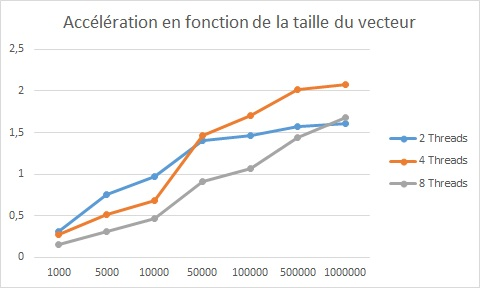
\includegraphics[width=12cm]{AccelerationTaille.jpg}
\captionof{figure}{}
\vspace{2cm}

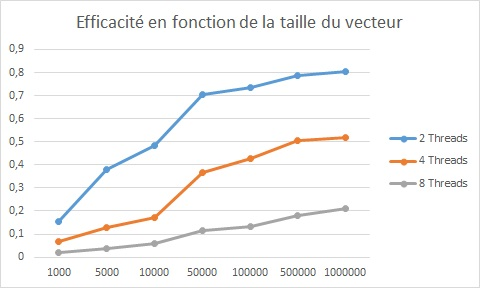
\includegraphics[width=12cm]{EfficaciteTaille.jpg}
\captionof{figure}{}

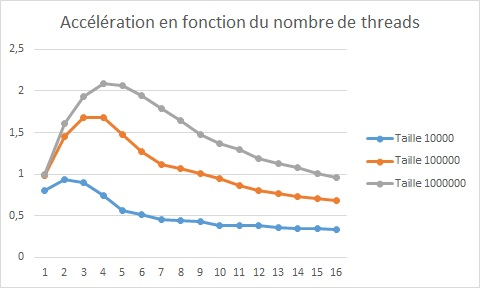
\includegraphics[width=12cm]{AccelerationThreads.jpg}
\captionof{figure}{}
\vspace{2cm}

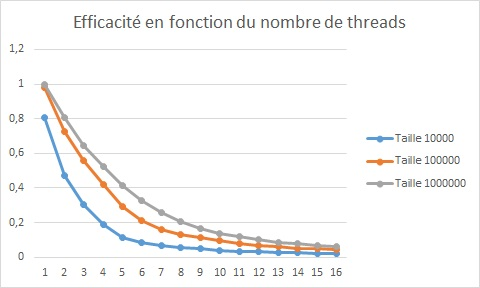
\includegraphics[width=12cm]{EfficaciteThreads.jpg}
\captionof{figure}{}
\end{center}

\section{Analyse des résultats}

\subsection*{Pour un nombre de threads fixé}

\subsubsection*{Figure 1}
On remarque que plus la taille du vecteur est grande et plus l'accélération est grande.

En effet, l'algorithme séquentiel va mettre de plus en plus de temps plus le vecteur est grand.

Alors que l'algorithme utilisant les threads va mettre de plus en plus de temps plus le vecteur est grand mais ce temps sera réparti entre les threads.\\

C'est donc pour cela que l'algorithme utilisant les threads sera plus rapide par rapport à l'algorithme séquentiel quand la taille du vecteur augmente.

On remarque également sur le graphique que pour une taille de vecteur inférieure à 50000, le tri sera plus rapide avec 2 threads puis après 50000, l'algorithme utilisant 4 threads a une meilleure accélération (En effet, la machine sur laquelle nous avons effectué nos tests possède 4 processeurs).\\

L'algorithme utilisant les threads ne devient vraiment plus rapide qu'à partir d'une taille de vecteur qui dépasse les 10000 (pour 2  threads), environ 20000 (pour 4 threads) et environ 100000 (pour 8 threads).

\subsubsection*{Figure 2}
On observe que plus la taille du vecteur augmente, plus l'efficacité augmente pour un nombre de threads fixe mais les courbes ont tendance à se stabiliser au dessus de 1000000 (L'efficacité tend vers un nombre différent selon le nombre de threads).\\

Pour une taille de vecteurs assez petite, l'efficacité des algorithmes utilisant les threads n'est pas notable.

En effet, le temps de la création des threads, de l'exécution de l'algorithme et de la synchronisation des threads, l'algorithme séquentiel a généralement déjà effectué son tri.\\

\subsection*{Pour une taille de vecteur fixé}

\subsubsection*{Figure 3}

On remarque un pic dans l'accélération. En effet on peut apercevoir que pour plusieurs tailles de vecteur fixes, il y a un nombre de threads pour lesquels l'algorithme est plus rapide.

Ici pour une taille de 10000, l'algorithme a une meilleure accélération avec 2 threads. Mais on remarque que peu importe le nombre de threads, l'algorithme séquentiel est plus rapide car aucune accélération ne dépasse 1.\\

Puis pour des tailles de vecteur plus conséquentes, on peut apercevoir que le "pic" est presque toujours vers 4 threads. Cela peut s'expliquer par le fait que la machine n'a que 4 processeurs et donc que 4 tâches peuvent s'éxécuter parallèlement.

\subsubsection*{Figure 4}

On remarque que plus on utilise de threads plus l'efficacité diminue car comme la machine utilisé n'a que 4 processeurs plus on va passer du temps à créer et synchroniser les processus. Le processeur va donc passer son temps à "switcher" les threads.

\end{document}